\documentclass[12pt]{article}

\usepackage{tikz}     %Better diagrams
  % tikz libraries
  \usetikzlibrary{matrix,positioning}

%Formatting
\usepackage[top=1.5in, bottom=1.5in, left=1in, right=1in]{geometry}
\setlength\parindent{0pt}
\setlength\parskip{.75em}


\begin{document}

\texttt{HLLL}=
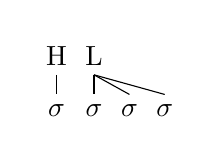
\begin{tikzpicture}[baseline=(m-1-1.base)]
  \matrix (m) [matrix of nodes, row sep=0.75em] {
    H        & L                              \\
    $\sigma$ & $\sigma$ & $\sigma$ & $\sigma$ \\
  };
  \draw (m-1-1.south) -- (m-2-1.north);
  \draw (m-1-2.south) -- (m-2-2.north);
  \draw (m-1-2.south) -- (m-2-3.north);
  \draw (m-1-2.south) -- (m-2-4.north);
\end{tikzpicture}
    
\texttt{LHHL}=
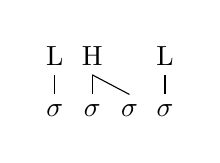
\begin{tikzpicture}[baseline=(m-1-1.base)]
  \matrix (m) [matrix of nodes, row sep=0.75em] {
    L        & H        &          & L        \\
    $\sigma$ & $\sigma$ & $\sigma$ & $\sigma$ \\
  };
  \draw (m-1-1.south) -- (m-2-1.north);
  \draw (m-1-2.south) -- (m-2-2.north);
  \draw (m-1-2.south) -- (m-2-3.north);
  \draw (m-1-4.south) -- (m-2-4.north);
\end{tikzpicture}

\texttt{0H00H0}=
\begin{tikzpicture}[baseline=(m-1-1.base)]
  \matrix (m) [matrix of nodes, row sep=0.75em] {
             &          & H        &          & H        &          \\
    $\sigma$ & $\sigma$ & $\sigma$ & $\sigma$ & $\sigma$ & $\sigma$ \\
  };
  \draw (m-1-3.south) -- (m-2-3.north);
  \draw (m-1-5.south) -- (m-2-5.north);
\end{tikzpicture}

\texttt{000F}=
\begin{tikzpicture}[baseline=(m-1-1.base)]
  \matrix (m) [matrix of nodes, row sep=0.75em] {
             &          &          & H        & L    \\
    $\sigma$ & $\sigma$ & $\sigma$ & $\sigma$        \\
  };
  \draw (m-1-4.south) -- (m-2-4.north);
  \draw (m-1-5.south) -- (m-2-4.north);
\end{tikzpicture}

    
    

\end{document}